% Figura cuerpo B2: con oferta vertical, la productividad mueve la producción y el dinero solo los precios
\documentclass[tikz,border=3pt]{standalone}
\usepackage[T1]{fontenc}
\usepackage[utf8]{inputenc}
\usepackage{amsmath}
\usetikzlibrary{arrows.meta,calc,positioning}
\begin{document}
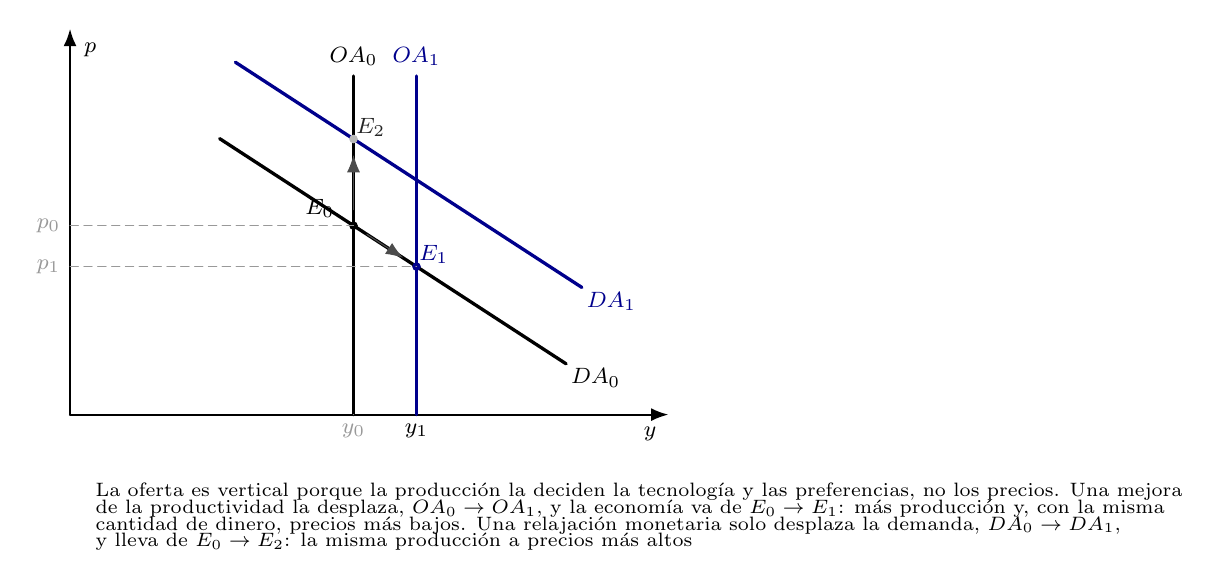
\begin{tikzpicture}[>={Latex[length=2.2mm]}, line cap=round, font=\footnotesize,
  eje/.style={->, thick},
  curva/.style={very thick},
  nueva/.style={very thick, blue!55!black},
  guia/.style={densely dashed, gray!80},
  pto/.style={circle, fill=black, inner sep=1.1pt}]
  \draw[eje] (0,0) -- (7.6,0) node[below left=1pt]{$y$};
  \draw[eje] (0,0) -- (0,4.9) node[below right=2pt]{$p$};
  % Ofertas verticales
  \draw[curva] (3.6,0) -- (3.6,4.3) node[above]{$OA_0$};
  \draw[nueva] (4.4,0) -- (4.4,4.3) node[above]{$OA_1$};
  % Demandas
  \draw[curva] (1.9,3.505) -- (6.3,0.645) node[below right=-3pt]{$DA_0$};
  \draw[nueva] (2.1,4.475) -- (6.5,1.615) node[below right=-3pt]{$DA_1$};
  % Equilibrios
  \node[pto] (E0) at (3.6,2.4) {};
  \node[inner sep=1pt] at (3.17,2.62) {$E_0$};
  \node[pto, fill=blue!55!black] (E1) at (4.4,1.88) {};
  \node[above right=-2pt of E1, inner sep=1pt, blue!55!black] {$E_1$};
  \node[pto, fill=gray!55] (E2) at (3.6,3.5) {};
  \node[above right=-2pt of E2, inner sep=1pt, gray!30!black] {$E_2$};
  \draw[guia] (0,2.4) node[left]{$p_0$} -- (3.6,2.4);
  \draw[guia] (0,1.88) node[left]{$p_1$} -- (4.4,1.88);
  \draw[guia] (3.6,0) -- (3.6,0) node[below]{$y_0$};
  \node[below] at (4.4,0) {$y_1$};
  \draw[->, gray!60!black, shorten >=4pt, shorten <=4pt] (E0) -- (E1);
  \draw[->, gray!60!black, shorten >=4pt, shorten <=4pt] (E0) -- (E2);
  \node[align=left, anchor=north west, font=\scriptsize] at (0.2,-0.75)
    {La oferta es vertical porque la producción la deciden la tecnología y las preferencias, no los precios. Una mejora\\[-2pt]de la productividad la desplaza, $OA_0\to OA_1$, y la economía va de $E_0\to E_1$: más producción y, con la misma\\[-2pt]cantidad de dinero, precios más bajos. Una relajación monetaria solo desplaza la demanda, $DA_0\to DA_1$,\\[-2pt]y lleva de $E_0\to E_2$: la misma producción a precios más altos};
\end{tikzpicture}
\end{document}
